\documentclass[a4paper,10pt]{article}
\setlength{\parindent}{0ex}
\setlength{\parskip}{1.5ex}
\usepackage[dvips]{graphicx}
\usepackage {epsfig}
\usepackage[a4paper, hmargin=15mm, vmargin=20mm, nohead]{geometry}

\begin{document}
\newcommand{\marks}[1]
{\begin{flushright}{\bf (#1 marks)}\end{flushright}}

{\centering \large \bf THE UNIVERSITY OF WAIKATO\\}
{\centering \large \bf Department of Computer Science\\[0.5cm]}

{\centering \large \bf COMP201Y Computer Systems 2003\\}
{\centering \large \bf Exercise 6 Test - 4th August 2003\\[0.3cm]}
{\centering \bf Worth 7\% --- Marked out of: 28\\[0.3cm]}
{\centering \bf Time allowed: 45 Min\\[1cm]}
\hrule

\begin{enumerate}
\item True/False answers. Indicate on your answer sheet if the
following statements are true or false.

\begin{enumerate}

\item Your exception handler checks for the interrupts it can handle.  If this
check fails it should jump to the system exception handler by loading its
address into the Exception Vector Register (\texttt{\$evec}).

\item When in autorestart mode, the timer will reload the value of the Timer
Count Register and start counting down again after every
interrupt it generates is acknowledged.

\item All exceptions are disabled on the WRAMP processor by setting the
Interrupt Enable bit of the CPU Control Register (\texttt{\$cctrl}) to zero.

\item When \texttt{'rfe'} instruction is executed the next instruction executed is at the address
held in the Exception Address Register (\texttt{\$ear}) register.

\item When an \texttt{'rfe'} instruction is executed the Kernel/User Mode bit of
CPU Control Register (\texttt{\$cctrl}) is set to zero.

\end{enumerate}

\marks{5}

\item When an interrupt occurs on a WRAMP processor, what values are loaded in to the
following bits/registers

\begin{enumerate}

	\item The program counter?
	
	\item The Interrupt Enable bit of the CPU Control Register
	(\texttt{\$cctrl})?
	
	\item General Purpose Register Thirteen (\texttt{\$13})?

\end{enumerate}

\marks{3}

\item Provided in Figure~\ref{code:badack} is some code which should
use the REX board timer to provide an interrupt once per second. Each
time an interrupt occurs an \texttt{'X'} should be printed. When the code is
executed however, no \texttt{X}'s are displayed on the Terminal.  Using the
Timer specifications given in Appendix~\ref{appen:timer}:

\label{ques:badack}

\begin{enumerate}
\item What is the error in the code that causes this problem ?
\marks{1}

\item Explain why this error results in the above behaviour.
\marks{2}

\item State the changes that you would make to ensure the code worked
as it should. You should provide the line numbers of any code that you
would change or the location that you would insert any new code into.
\marks{2}

\end{enumerate}

\begin{figure}[p]
\begin{footnotesize}
\begin{center}
\begin{tabular}{|p{12cm}|}
\hline
\begin{verbatim}
   1:  .text
   2:  .global main
   3:  main:
   4:    # Get the old exception vector
   5:    movsg  $2, $evec
   6:    # ...and save it.
   7:    sw     $2, old_vector($0)
   8:    # Get the address of my exception handler
   9:    la     $2, handler
  10:    # put it into the exception vector register
  11:    movgs  $evec, $2
  12:
  13:    # Get the CPU control register
  14:    movsg  $2, $cctrl
  15:    # Mask out all interrupts
  16:    andi   $2, $2, 0xf
  17:    # Enable IRQ2 (Timer) and Interrupt Enable.
  18:    ori    $2, $2, 0x42
  19:    # Replace the CPU control register
  20:    movgs  $cctrl, $2
  21:    
  22:    # Acknowledge any outstanding timer interrupts
  23:    sw     $0, 0x72003($0)
  24:    # Setup the delay between interrupts to 1 second.
  25:    addi   $2, $0, 2400
  26:    sw     $2, 0x72001($0)
  27:    # Setup the timer to Autostart 
  28:    addi   $2, $0, 0x2
  29:    sw     $2, 0x72000($0)
  30:    
  31:  loop:   # Begin our main loop
  32:    # Read from the switches
  33:    lw     $2, 0x73000($0)
  34:    # Display the value on the SSDs
  35:    sw     $2, 0x73003($0)
  36:    srli   $2, $2, 4
  37:    sw     $2, 0x73002($0)
  38:    j      loop
  39:    
  40:  handler:
  41:    # Check the cause of the exception
  42:    movsg  $13, $estat
  43:    andi   $13, $13, 0xffb0
  44:    
  45:    # If timer then go to handle_interrupt
  46:    beqz   $13, handle_interrupt
  47:    
  48:    # Otherwise go to the system exception handler
  49:    lw     $13, old_vector($0)
  50:    jr     $13
  51:    
  52:  handle_interrupt:
  53:    # acknowledge interrupt
  54:    sw $0, 0x72003($0)
  55:	 
  56:  serial_check:
  57:    # Check the serial status register
  58:    lw     $13, 0x71003($0)
  59:    # Check the transmit data sent bit
  60:    andi   $13, $13, 0x2
  61:    # Wait for the previous character to be sent
  62:    beqz   $13, serial_check
  63:    # Send an 'X' to the terminal
  64:    addi   $13, $0, 'X'
  65:    sw     $13, 0x71000($0)
  66:    
  67:    # Return to the mainline
  68:    rfe
  69:
  70:  .data
  71:  old_vector:
  72:    .word  0
\end{verbatim}
\\ \hline
\end{tabular}
\end{center}
\end{footnotesize}
\caption{Code for Question~\ref{ques:badack}}
\label{code:badack}
\end{figure}

\clearpage
\item In order to allow the main loop to perform some other task, the code in
Figure~\ref{code:badack} needs to be modified so that the switch value is only
read and displayed to the SSDs when a switch position is changed.   Using the
specifications of the Parallel Interface given in Appendix~\ref{appen:parallel},
the CPU Control Register given in Appendix~\ref{appen:cctrl} and the Exception
Status Register give in Appendix~\ref{appen:estat}:

\begin{enumerate}

\item Write new setup code to enable interrupts from the Parallel Interface on
switch changes, as well as interrupts from the Timer.  Be sure to correctly set
up the timer.

\marks{5}

\item Write a new handler to check for interrupts from both the Parallel
Interface and the Timer.  It should jump to \texttt{handle\_timer\_interrupt} on
an interrupt from the Timer and jump to \texttt{handle\_parallel\_interrupt} on
an interrupt from the Parallel Interface.

\marks{5}

\item Write the code for the \texttt{handle\_parallel\_interrupt} routine to read
the value of the switches, display them on the SSDs, acknowledge the parallel interrupt,
and then return to the main loop.

\marks{5}

\end{enumerate}

\end{enumerate}

\newpage
\appendix
\section{Programmable Timer}
\label{appen:timer}

The Programmable Timer on the REX board provides for generation of
interrupts at time intervals from about 1ms to 30s, with a resolution
of around 0.5ms.

The timer has an internal 16 bit register. This register is
decremented at a constant rate of 2400Hz. Once this register reaches
\texttt{0x0000} an interrupt is triggered. The starting value for the
timer is controlled by altering the value in the timer load register.

The timer can be configured to automatically reload the starting count
value and continue counting immediately after it expires.

The programmers view of the timer consists of four registers.  The
names of these registers and their addresses, expressed as offsets
from the base address, are provided in
Table~\ref{table:timer_offsets}.  The base address for the timer is
\texttt{0x72000}.

\begin{table}[h]
\begin{center}
\begin{tabular}{|l|c|}
\hline
\textbf{Register name} & \textbf{Offset} \\
\hline
Timer Control Register & 0 \\
\hline
Timer Load Register & 1 \\
\hline
Timer Count Register & 2 \\
\hline
Timer Interrupt Acknowledge Register & 3 \\
\hline
\end{tabular}
\caption{Timer Register Offsets}
\label{table:timer_offsets}
\end{center}
\end{table}


\subsection{Timer Control Register}

The Timer Control Register is a read/write register, that allows the
user to enable and control aspects of the timer operation. The timer
has two primary modes of operation, automatic restart and single-shot
mode. If the timer is set to automatic restart, as soon as the timer
expires, an interrupt is triggered and the timer immediately starts
counting down again. In single-shot mode the timer will copy the value
from the timer load register only once when the timer is enabled and
will count down to zero. Once the timer reaches zero an interrupt will
be triggered and the timer will be disabled.

\begin{figure}[h]
\begin{center}
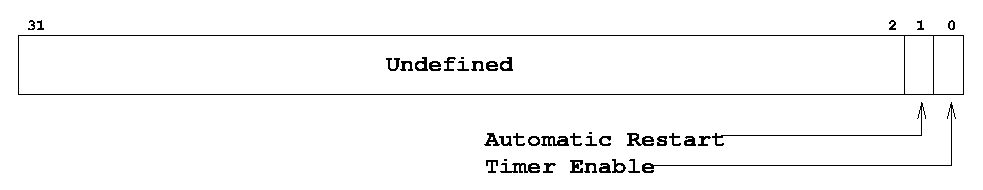
\includegraphics[width=0.8\textwidth]{timer_cr.eps}
\caption{The Timer Control Register}
\label{timer_cr_pic}
\end{center}
\end{figure}

\subsection{Timer Load Register}

The Timer Load Register is a read/write register. This register allows
the user to specify the starting count value. The starting count value
is a 16 bit value with the upper 16 bits being ignored.

\subsection{Timer Count Register}

The Timer Count Register is a read-only register. Reading from this
register returns the current value in the 16 bit internal count
register.

\subsection{Timer Interrupt Acknowledge Register}

The Interrupt Acknowledge Register is a read/write register. This
register allows a program to detect a timer overrun as as well as
acknowledge interrupts that have been dealt with.

The overrun detected bit will be set if the timer is set to automatic
restart and the timer expired again before the previous interrupt was
acknowledged. This allows a program to detect if it is unable to
service the timer interrupt fast enough.

The overrun bit must be manually reset by writing a `\texttt{0}' to
it's location.

\begin{figure}[h]
\begin{center}
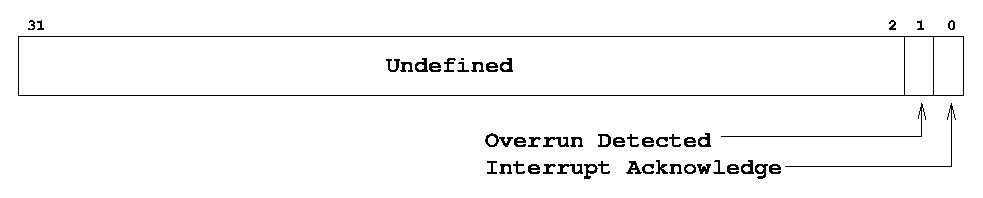
\includegraphics[width=0.8\textwidth]{timer_iack.eps}
\caption{The Timer Interrupt Acknowledge Register}
\label{timer_iack_pic}
\end{center}
\end{figure}

eg. If the value `\texttt{11}' was read from the interrupt acknowledge
register we could determine that the timer has overrun since we last
acknowledged an interrupt. If `\texttt{00}' was written to the timer
interrupt acknowledge register we will acknowledge any outstanding
interrupts and ensure the overrun bit is reset to zero.

\subsection{Timer Example}

To configure the timer to interrupt at a specific period the first
step is to calculate the timer load value. This value can be
calculated simply by multiplying the timer frequency by the required
time between interrupts. For example, if we want the timer to generate
an interrupt once every ten seconds we would calculate it as follows:

\begin{center}
Timer Load = 2400Hz * 10s = 24000
\end{center}

Some simple code to initialise the timer to automatically restart and
to interrupt once every ten seconds is given in
Figure~\ref{code:timer_init}.

\begin{figure}[h]
\begin{footnotesize}
\begin{center}
\begin{tabular}{|p{8cm}|}
\hline
\begin{verbatim}
            . . .
           # Make sure there are no old interrupts
           # still hanging around
           sw   $0, 0x72003($0)
           # Put our auto load value in
           addi $11, $0, 24000
           sw   $11, 0x72001($0)
           # Enable the timer and autorestart
           addi $11, $0, 0x3
           sw   $11, 0x72000($0)
            . . .
\end{verbatim}
\\
\hline
\end{tabular}
\end{center}
\end{footnotesize}
\caption{Simple Timer Initialisation}
\label{code:timer_init}
\end{figure}


\newpage
\section{Parallel Interface}
\label{appen:parallel}
The parallel interface on the REX board provides an input interface
from a bank of 8 on-off switches and two momentary push-buttons, as
well as an output interface to two LED Seven Segment Displays (SSDs).
Parallel interrupts, if enabled, will be generated on any switch or
push-button state change.

The programmers view of the parallel interface consists of six
registers.  The names of these registers and their addresses,
expressed as offsets from the base address, are provided in
Table~\ref{table:parallel_offsets}. The base address for the parallel
port is \texttt{0x73000}.

\begin{table}[h]
\begin{center}
\begin{tabular}{|l|c|}
\hline
\textbf{Register name} & \textbf{Offset} \\
\hline
Parallel Switch Register & 0 \\
\hline
Parallel Push Button Register & 1 \\
\hline
Parallel Left SSD Register & 2 \\
\hline
Parallel Right SSD Register & 3 \\
\hline
Parallel Control Register & 4 \\
\hline
Parallel Interrupt Acknowledge Register & 5 \\
\hline
\end{tabular}
\caption{Parallel Port Register Offsets}
\label{table:parallel_offsets}
\end{center}
\end{table}



\subsection{Parallel Switch Register}

The switch register is a read-only register. A read from this register
returns a bit pattern with bits set corresponding to the switches that
are on.

\begin{figure}[h]
\begin{center}
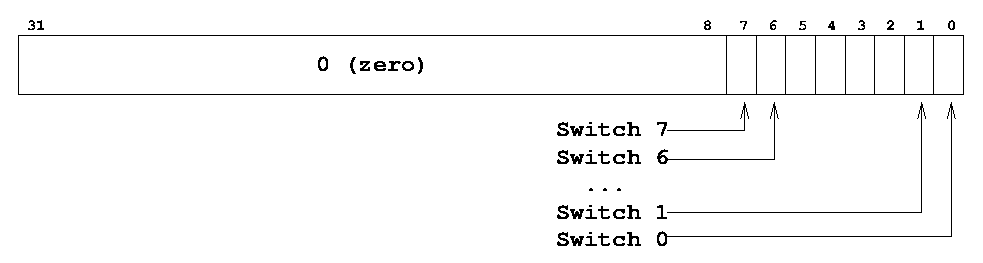
\includegraphics[width=0.8\textwidth]{switch_reg.eps}
\caption{The Switch Register}
\label{switch_reg_pic}
\end{center}
\end{figure}


\subsection{Parallel Push Button Register}

The push button register is a read-only register. A read from this
register returns a bit pattern in the low order 2 bits corresponding
to the push buttons that are currently being depressed.

\begin{figure}[h]
\begin{center}
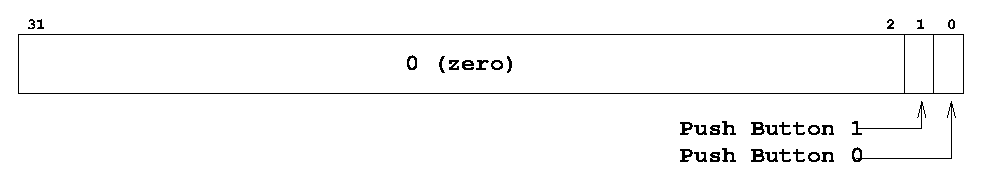
\includegraphics[width=0.8\textwidth]{button_reg.eps}
\caption{The Push Button Register}
\label{button_reg_pic}
\end{center}
\end{figure}

\subsection{Parallel Left and Right SSD Registers}

The Left and Right SSD Registers are read/write registers. These
registers contain the value to be displayed on their respective Seven
Segment Display. 

If the hexadecimal to seven-segment decode bit is enabled in the
parallel control register, four bits of input will be decoded into a
single hexadecimal digit and displayed on the seven-segment display.

If the hexadecimal to seven-segment decode bit is turned off, then
each segment can be individually controlled by a single bit of the
input. The displays are made up of seven segments and a decimal point.
The first eight bits of input turn on the segments as shown in
Figure~\ref{fig:ssd}.

\begin{figure}[h]
\begin{center}
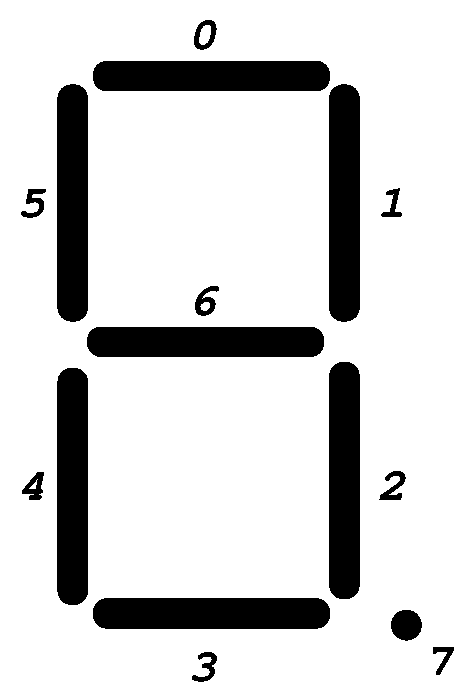
\includegraphics[width=0.12\textwidth]{ssd.eps}
\caption{Seven-segment display bit encoding}
\label{fig:ssd}
\end{center}
\end{figure}

\subsection{Parallel Control Register}

The Parallel Control Register is a read/write register, which allows
for control over the parallel interface.

\begin{figure}[h]
\begin{center}
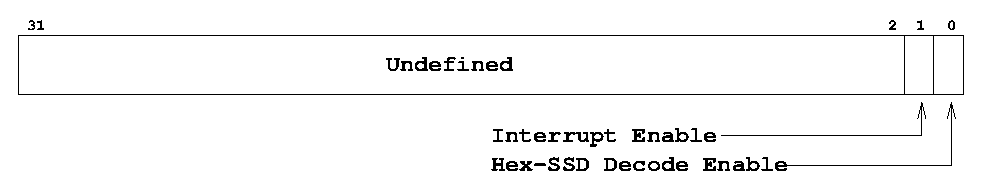
\includegraphics[width=0.8\textwidth]{parallel_cr.eps}
\caption{The Parallel Control Register}
\label{parallel_cr_pic}
\end{center}
\end{figure}

eg. To enable interrupts on switch changes and force hex-SSD decoding
on the displays, a value of `\texttt{11}' would be written to
the parallel control register.

\subsection{Parallel Interrupt Acknowledge Register}

The Interrupt Acknowledge Register is a read/write register. This
register allows a program to determine the parallel port interrupt
status as well as acknowledge interrupts that have been dealt with.

\begin{figure}[h]
\begin{center}
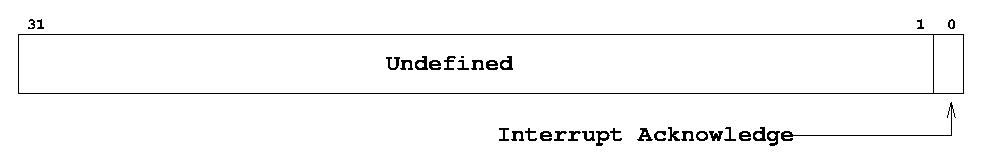
\includegraphics[width=0.8\textwidth]{parallel_iack.eps}
\caption{The Parallel Interrupt Acknowledge Register}
\label{parallel_iack_pic}
\end{center}
\end{figure}

eg. To acknowledge an outstanding parallel port interrupt `\texttt{0}'
would be written to the parallel interrupt acknowledge register.

\newpage
\section{\$cctrl - CPU Control Register}
\label{appen:cctrl}
\begin{figure}[h]
\begin{center}
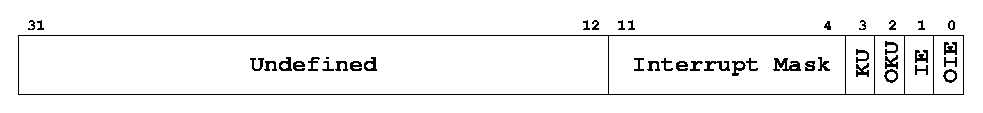
\includegraphics[width=\textwidth]{cctrl.eps}
\caption{\$cctrl - CPU Control Register}
\label{cctrl_pic}
\end{center}
\end{figure}

The CPU control register controls almost all of the functionality
related to the WRAMP exception mechanism. There are three main
sections of this register:

\begin{itemize}
\item Interrupt Enable (IE)
\item Kernel/User Mode (KU)
\item Interrupt Mask
\end{itemize}

\subsection{Interrupt Enable}

This flag provides a global interrupt enable. If this location is set
to `\texttt{0}' then no interrupts can be triggered. This flag
\emph{only} affects external interrupts. There is no way on the WRAMP
processor to disable internal exceptions.

Interrupts that occur while the global interrupt enable is turned off
will be held back. As soon as interrupts are again enabled by writing
a `\texttt{1}' into this location the interrupt mask will be consulted
to discover if that specific interrupt is enabled. See
Section~\ref{sec:imask} for more information about the interrupt mask.

The CPU will automatically set the IE bit to `\texttt{0}' whenever an
exception of any type occurs. This prevents the exception handler
from being interrupted by another interrupt.

\subsection{Interrupt Mask}
\label{sec:imask}

This provides a way to selectively turn on and off individual external
interrupts. This field has a bit corresponding to each of the eight
possible external interrupts (IRQ0 - IRQ7). Bit 4 of the CPU control
register corresponds to IRQ0, bit 5 to IRQ1 and so on.

The interrupt mask field is only consulted if the global interrupt
enable (IE) flag is set. If an interrupt occurs and the global
interrupt flag is set but the individual interrupt mask is disabled
then the interrupt will be held back. As soon as both the global
interrupt enable and the specific interrupt mask bits are set then the
interrupt will occur.

\subsection{Kernel User Mode}

The WRAMP CPU has two modes of operation, kernel and user mode. If
there is a `\texttt{1}' in the KU bit the CPU is in kernel mode. If
the KU bit is set to `\texttt{0}' then the CPU is in user mode. 

If the CPU is running in kernel mode it will execute all instructions and
allow access to all areas of memory. If the CPU is running in user
mode programs are not allowed to use any of the three instructions
which deal with the special register file (\texttt{movsg, movgs, rfe})
and may not be able to access all memory locations. If a program
running in user mode attempts to use one of these instructions, or to
access protected memory the CPU will cause a General Protection Fault
exception.

The CPU will automatically set the KU bit to `\texttt{1}' whenever an
exception of any type occurs. This allows the exception handler to
operate in kernel mode, allowing it full access to all instructions
and memory locations.


\newpage
\section{\$estat - Exception Status Register}
\label{appen:estat}

\begin{figure}[h]
\begin{center}
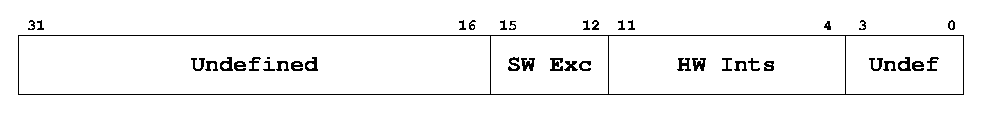
\includegraphics[width=\textwidth]{estat.eps}
\caption{\$estat - Exception Status Register}
\label{estat_pic}
\end{center}
\end{figure}

The exception status register provides the exception handler with the
ability to discover what exceptions caused it to be called. The
exception status register has a single bit flag for each external IRQ
line. Bit 4 of the status register corresponds to IRQ0, bit 5 to IRQ 1
and so on. In addition to the eight external interrupt sources the
status register also provides the status for the four CPU internal
exception sources.

The full list of all exception sources and their related status
register bit is given in Table~\ref{table:sta_loc}.

\begin{table}[h]
\begin{center}
\begin{tabular}{|l|c|}
\hline
\textbf{Exception source} & \textbf{Bit location} \\
\hline
IRQ0 & 4 \\
\hline
IRQ1 - User Interrupt Button & 5 \\
\hline
IRQ2 - Timer Interrupt & 6 \\
\hline
IRQ3 - Parallel Interrupt & 7 \\
\hline
IRQ4 - Serial Port 1 Interrupt & 8 \\
\hline
IRQ5 - Serial Port 2 Interrupt & 9 \\
\hline
IRQ6 & 10 \\
\hline
IRQ7 & 11 \\
\hline
General Protection Fault Exception & 12 \\
\hline
System Call Exception & 13 \\
\hline
Breakpoint Exception & 14 \\
\hline
Arithmetic Exception & 15 \\
\hline
\end{tabular}
\caption{Exception Status Register Fields}
\label{table:sta_loc}
\end{center}
\end{table}

\end{document}




